\documentclass[a4paper,twocolumn]{jsarticle}
\usepackage[dvipdfm,left=1.0cm,right=1.0cm,top=1.0cm,bottom=1.0cm]{geometry}
\usepackage[dvipdfmx]{graphicx}
\usepackage{tabularx}
\pagestyle{empty}
\usepackage{ascmac}
\usepackage{here}
\usepackage{scalefnt}
%%%%%%%%%%%%%%%%%%%%%%%%%%%%%%%%%%%%%%%%%%%%%%%%%%%%%%%%%%%%%%%%%%%%%%%%%%%%%%%%
% ここを各自編集
\newcommand{\jtitle}{計算問題の特徴分布に基づく類題選出による自己学習支援 }
\newcommand{\jauthor}{% 著者(日)
プログラミング言語研究室 S152114 宮地 雄也}


%%%%%%%%%%%%%%%%%%%%%%%%%%%%%%%%%%%%%%%%%%%%%%%%%%%%%%%%%%%%%%%%%%%%%%%%%%%%%%%%

\begin{document}

\twocolumn[
\begin{center}%
  {\Large \bf \jtitle \par}
  \vskip 2ex
  {\large \begin{tabular}{c} \jauthor \end{tabular}\par}
  \vskip 2ex
\end{center}
]

%%%%%%%%%%%%%%%%%%%%%%%%%%%%%%%%%%%%%%%%%%%%%%%%%%%%%%%%%%%%%%%%%%%%%%%%%%%%%%%%
% ここから本文
%%%%%%%%%%%%%%%%%%%%%%%%%%%%%%%%%%%%%%%%%%%%%%%%%%%%%%%%%%%%%%%%%%%%%%%%%%%%%%%%

\section{はじめに} \label{sec:intro}

昨今,小・中学生の理系離れが問題視されている
この要因の一つに,数学は一つの計算方法が様々な分野に横断していくことが一度,苦手を生んでしまったらそこからの分野の理解度が下がり,各単元のちょっとした積み残しが後々,尾を引いている.この状況を打破するには子供一人一人の苦手と向き合い,苦手と感じる前に理解させていくしかない.
この打開策として,IT技術駆使した個人別最適化学習に注目が集まっている,
しかし,教育の情報は,生徒の情報と結びついている個人情報なためオープン化できず,現在でているサービスでは各サービス利用者の利用状況からデータを取得し,その運用に利用しているため一部の大手企業が情報を独占している.
そこで個人の統計データではなく,解く数式の方に着目し,計算式自体の特徴を抽出し,間違えた問題と同様の特徴を持つ問題が復習する類題として最適なのではないかという仮定のもと,本論文では数式の特徴を掴むために自然言語処理の分野で使用される分散表現を適用し,さらに再帰ニューラルネットワークを用いて数式ベクトルを作り出すことを目標とし,そのベクトルを用いて実際に復習問題推定を行った.

\section{解決手法} \label{sec:method}

数式を分布化する際,そのベクトルの中に数式の特徴を入れ込んだベクトルを生成する手法が確立していない.しかしながら自然言語の分野では単語を効率よく埋め込み層に変換するWord2Vecという手法が結果を残している.(文献\cite{SkipCBOW})
そこで本論文では数式の各文字,記号を単語のようにみなし,onehotベクトルを作成し,それを埋め込み層で特徴を踏まえた低次元ベクトルに変換したのち,系列変換モデルで読み込むことで低次元で数式の特徴を掴んだベクトルを生成できないかと考えた.

そこで本論文では数式をある一定のルールの中でテキスト化されている{\TeX}形式の数式を用いる.
本論文の目的としては系列変換の過程で用いれるEncoderからDecoderに渡す最終出力$h$を式ベクトルとしてみなす.図\ref{fig:EVS_Simple}にモデル模式図を掲載する

\begin{center}
  \begin{figure}[htb]
    \centering
    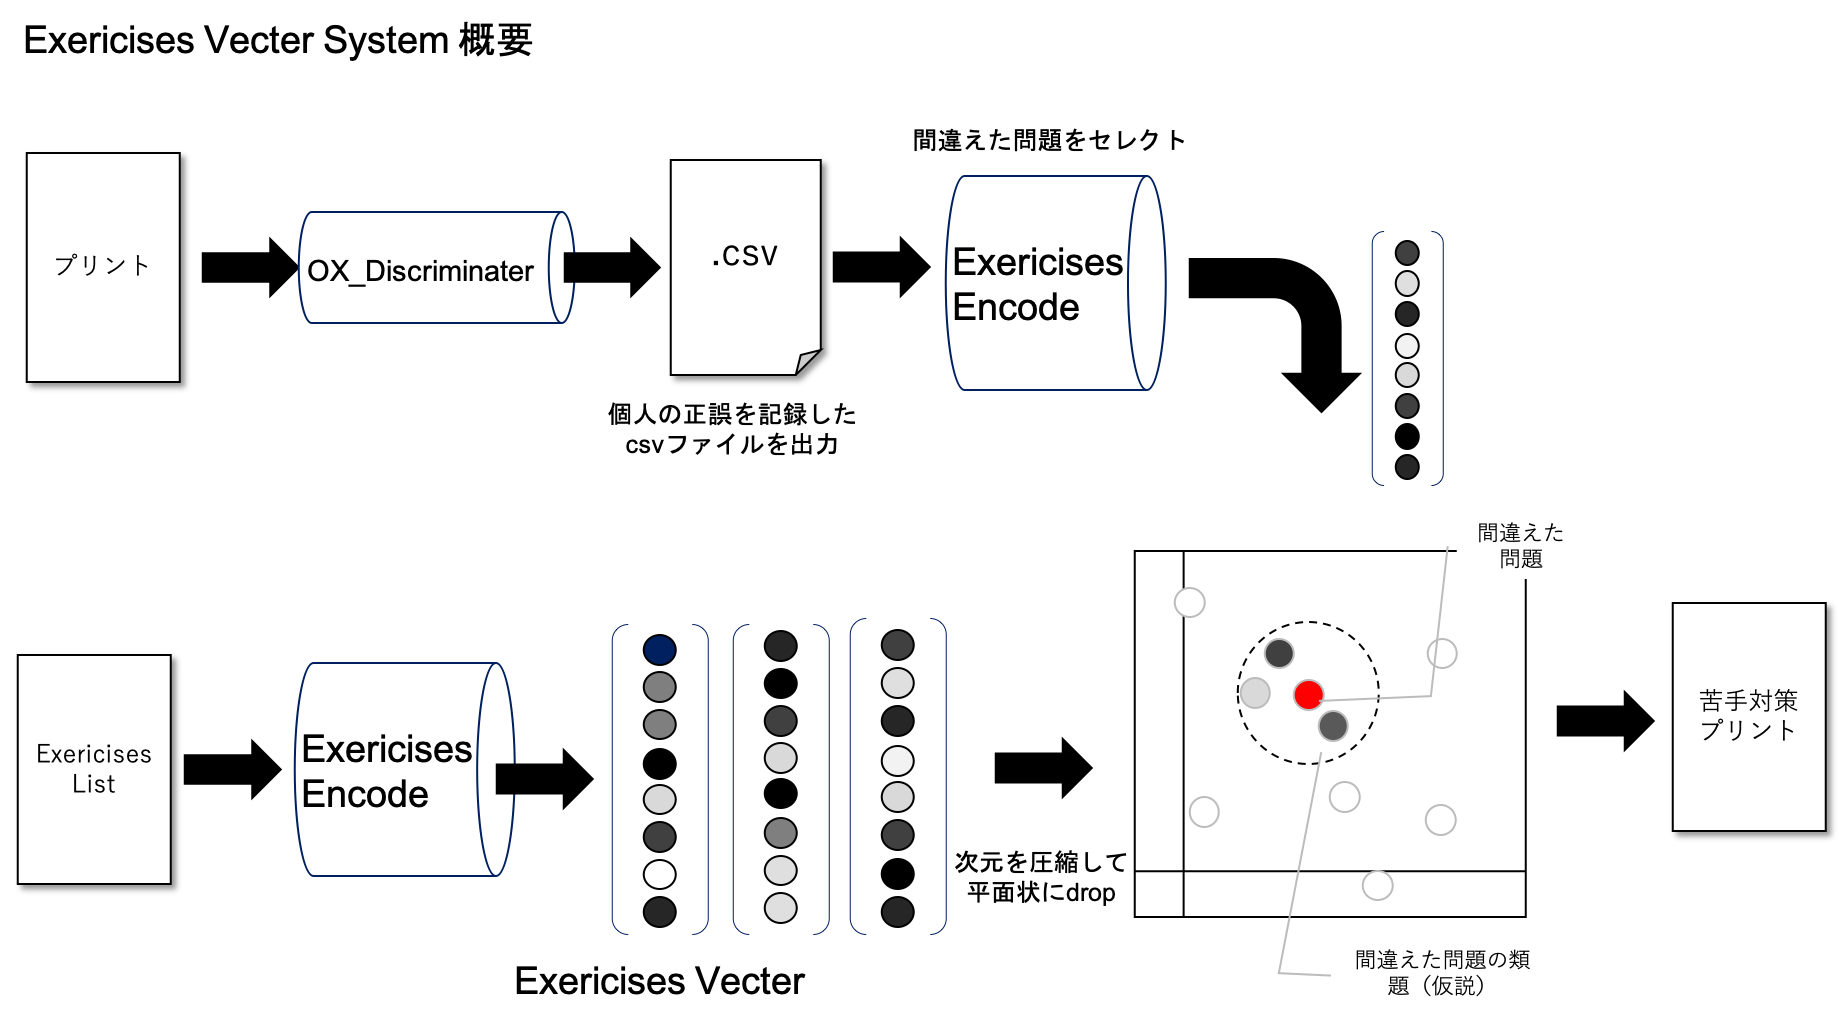
\includegraphics[width=0.8\linewidth]{image/EVS_Simpie.png}
    \caption{ExercisesEncoderは入力をベクトルに変換することを担う.}
    \label{fig:EVS_Simple}
  \end{figure}
\end{center}

より高い精度の分布を得るためには$h$の精度を高めていくモデルが必要となる.
実験するモデルは通常のLSTMで行う系列変換,双方向RNNを用いたbi-directionlモデル,通常Decoderが側で利用されるSkipConnectionの三種類をEncoderのモデルとした.
デコーダ側は通常のLSTMで行う系列変換で行うこととした.
Encorder側のモデル構成図を
図\ref{fig:seq2seq},図\ref{fig:bi-directionl Seq2seq},図\ref{fig:SkipSeq2seq}に示す.


\begin{figure}[htpb]
  \centering
  \begin{tabular}{c}

    \begin{minipage}{0.33\hsize}
      \centering
      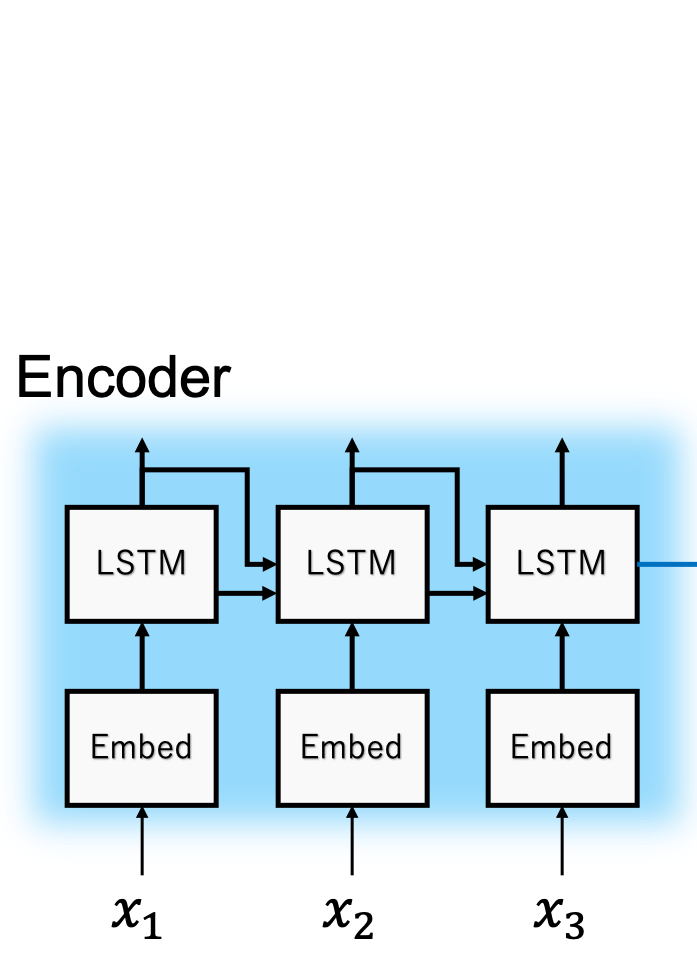
\includegraphics[width=\linewidth]{image/seq2seq_image_encoder.png}
      \caption{基本となるNormalEncoder}
      \label{fig:seq2seq}
    \end{minipage}

    \begin{minipage}{0.33\hsize}
      \centering
      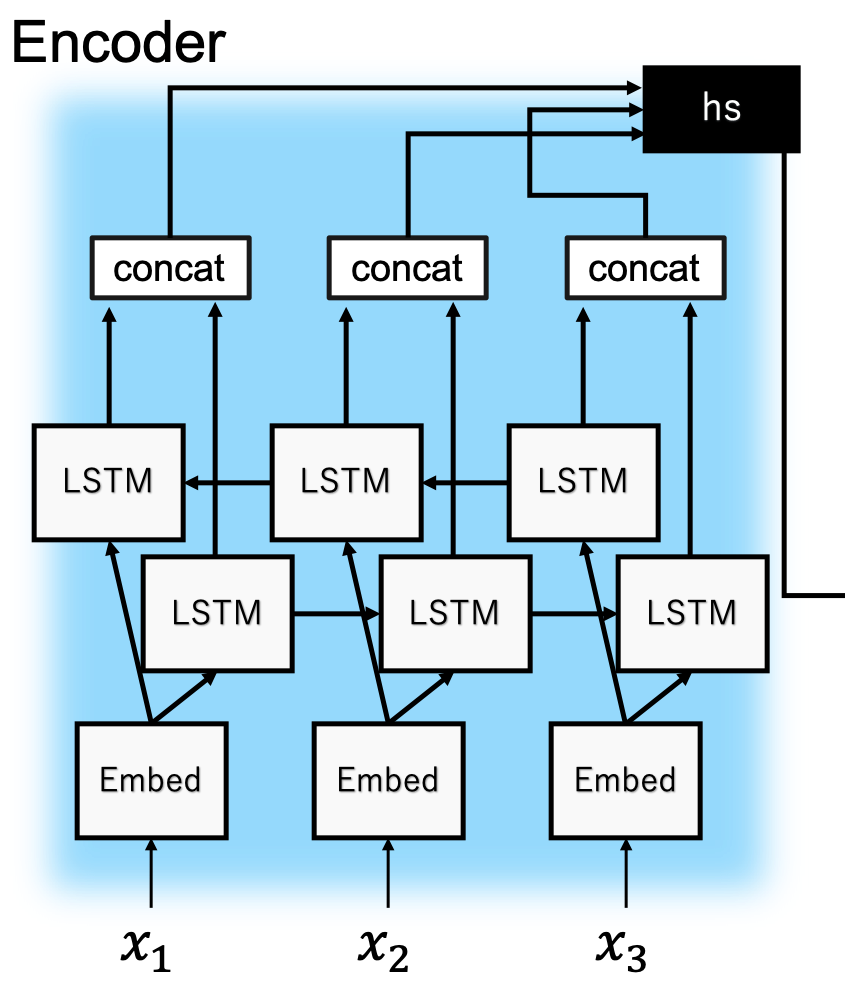
\includegraphics[width=\linewidth]{image/twinRNN_encoder.png}
      \caption{bi-directionl Encoder}
      \label{fig:bi-directionl Seq2seq}
    \end{minipage}

    \begin{minipage}{0.33\hsize}
      \centering
      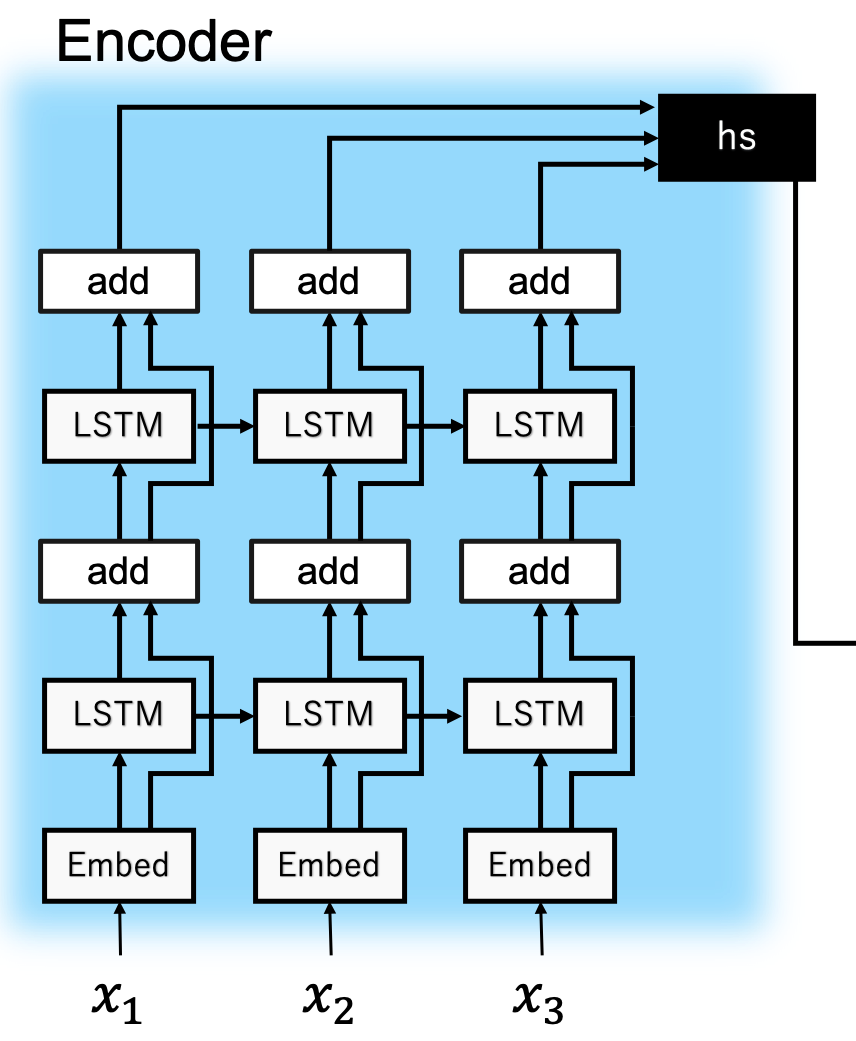
\includegraphics[width=\linewidth]{image/Skipconnect_encoder.png}
      \caption{Skip Encoder}
      \label{fig:SkipSeq2seq}
    \end{minipage}

    %--- 中央スペース

  \end{tabular}
\end{figure}

入力は$f,\{,\},(,),x,=,+,-,\dot,0,1,2,3,4,5,6,7,8,9,<EOS>,<UNK>$の22種類で$<EOS>$は数式の始まりを表し,$<UNK>$は予想される出力が入力の22次元内に存在しない時,または未知の入力に対して対応するものとする.

実験にて確認を行ったネットワーク構成を\ref{tb:network_collection}に示す.
\begin{table}[H]
  \centering
  \caption{ネットワーク構成}
  \begingroup
  \scalefont{0.8}
  \begin{tabular}{|l|c|r|r|r|} \hline
    モデル & 入力サイズ & Encoderの出力サイズ & LSTM層の数 \\ \hline \hline
    Normal& 22 & 200              &      1 \\
    &          & 200              &      4 \\
    &          & 200              &      8 \\
    &          & 500              &      1 \\
    &          & 500              &      4 \\
    &          & 500              &      8 \\ \hline \hline
    SkipConnect& 22       & 200              &      1 \\
    &          & 200              &      4 \\
    &          & 200              &      8 \\
    &          & 500              &      1 \\
    &          & 500              &      4 \\
    &          & 500              &      8 \\ \hline \hline
    BiDirectional& 22       & 200 &      1 \\
    &          & 500              &      1 \\ \hline
  \end{tabular}

  \label{tb:network_collection}
  \endgroup
\end{table}


\section{実験結果} \label{sec:result}

以下,実験で得た式のベクトルをPCAを用いて二次元に次元削減したものである.
学習データとして用いたのは以下の20個の式である.
\begin{enumerate}
  \item \verb#x+5=8
  \item \verb#5x-7=4
  \item \verb#3.6+x=-1.4
  \item \verb#3x-4=-5x+5
  \item \verb#\frac{7}{2}x+9=6
  \item \verb#3(2x-1)=9
  \item \verb#\frac{3}{7}x+2=\frac{6}{7}
  \item \verb#-\frac{4}{7}x+3=-\frac{1}{7}x
  \item \verb#\frac{x+1}{3}+\frac{2x+1}{2}=\frac{3x-4}{2}
  \item \verb#-4x+9=1
  \item \verb#5x-9=10
  \item \verb#7.2x-4=2.2x+9
  \item \verb#3(x-4)=7x-10
  \item \verb#\frac{3}{7}x-3=-5
  \item \verb#-\frac{9}{8}x-4=-3x
  \item \verb#\frac{x-5}{4}+6=\frac{5}{2}
  \item \verb#\frac{2x+1}{5}=\frac{x-5}{4}
  \item \verb#0.8x-(0.01x-2)=0.03x-2
  \item \verb#-10x-5=8
  \item \verb#5x+10=1
\end{enumerate}
以下,実験の結果の抜粋である.

\begin{center}
  \begin{figure}[htb]
    \centering
    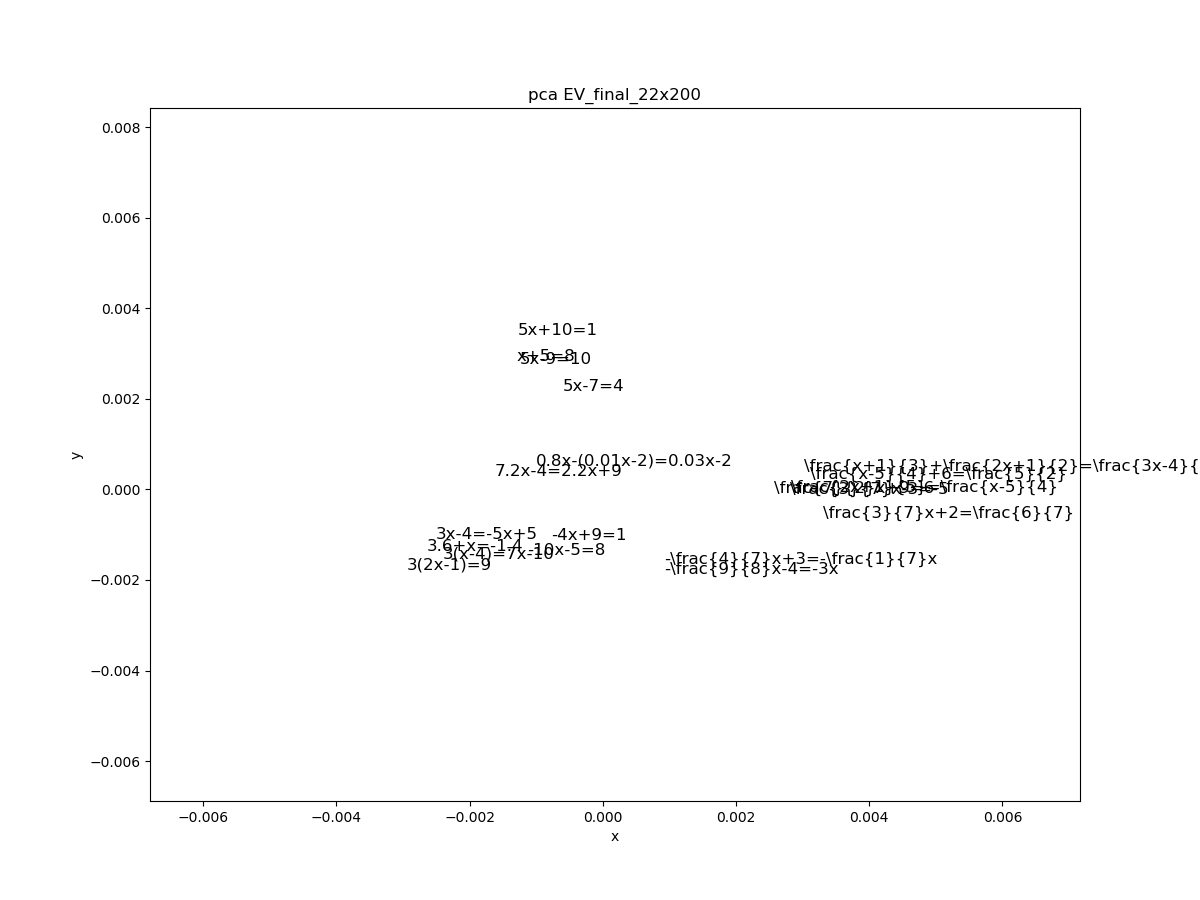
\includegraphics[width=0.7\linewidth]{image/pca_formula_EV_final_22x200_1_Wed_Feb_06_03:50:09.png}
    \caption{Normal LSTM1層200次元 学習データ}
    \label{fig:Simple}
  \end{figure}
\end{center}

\begin{center}
  \begin{figure}[htb]
    \centering
    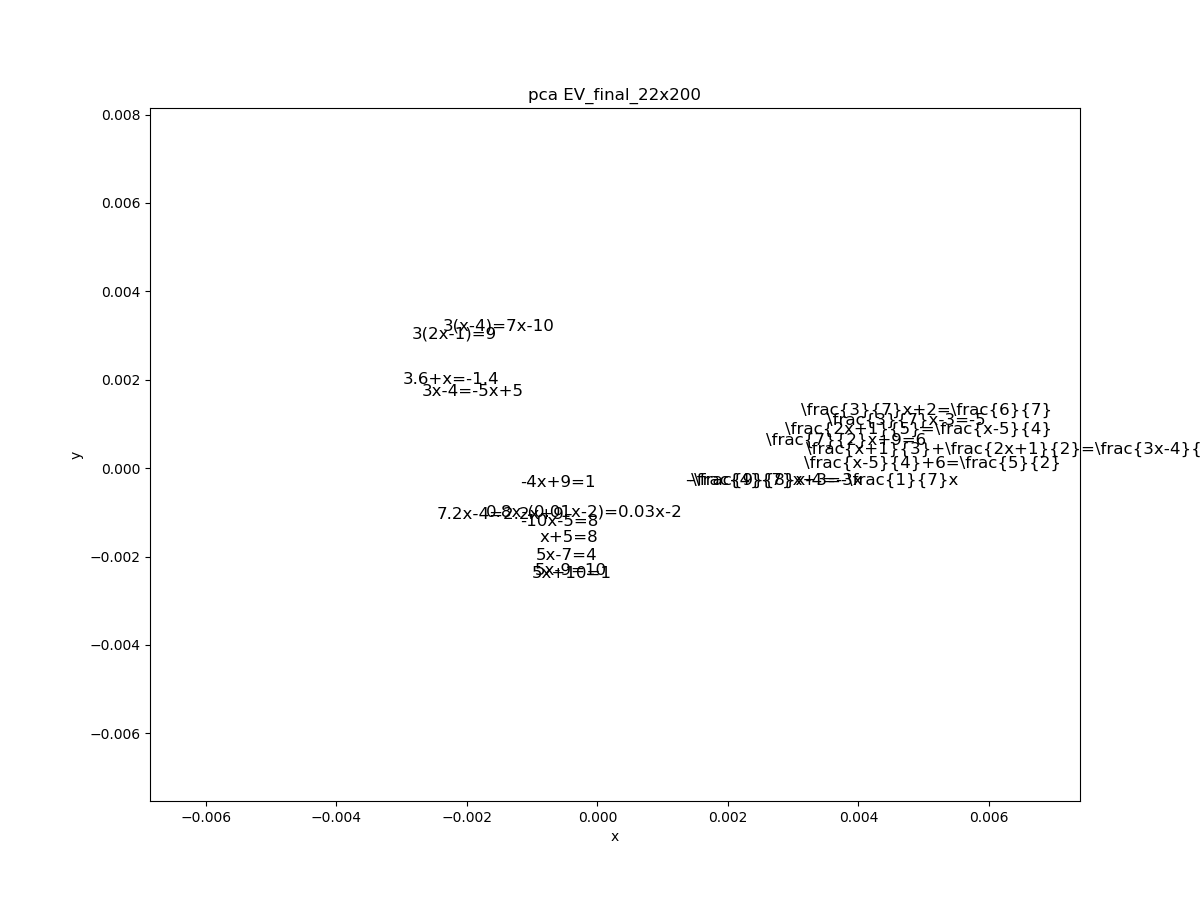
\includegraphics[width=0.7\linewidth]{image/pca_formula_EV_final_22x200_1_Wed_Feb_06_04:42:56.png}
    \caption{Skipconnect:LSTM4層200次元 学習データ}
    \label{fig:Skip4layer}
  \end{figure}
\end{center}

\begin{center}
  \begin{figure}[htb]
    \centering
    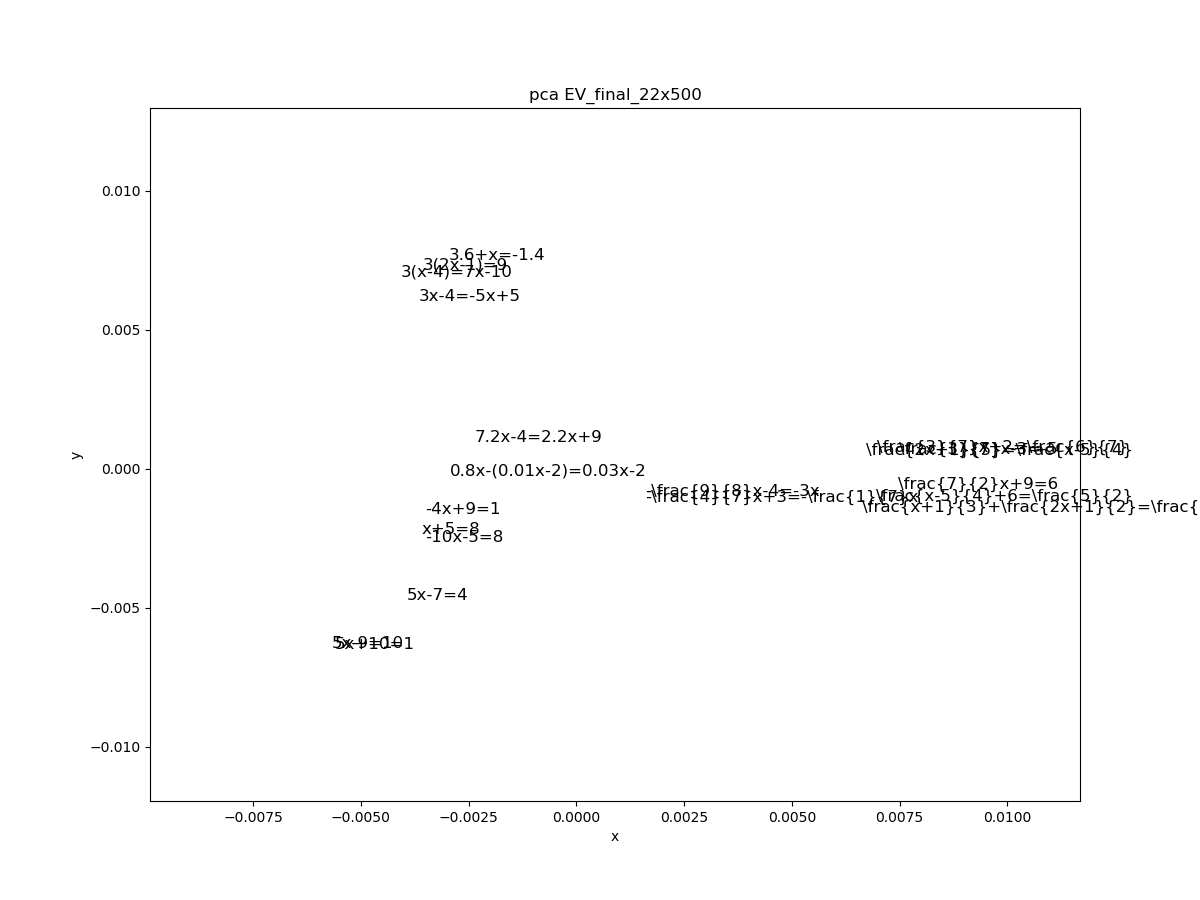
\includegraphics[width=0.7\linewidth]{image/pca_formula_EV_final_22x500_1_Wed_Feb_06_04:57:54.png}
    \caption{BiDirection:LSTM4層500次元 学習データ}
    \label{fig:Bi500layer4}
  \end{figure}
\end{center}

図\ref{fig:Simple},図\ref{fig:Skip4layer},図\ref{fig:Bi500layer4}のどれもが同系列そうな問題が近い分布となった.特に図\ref{fig:Skip4layer}は分数の中でも符号でも分かれており,高精度でベクトル化に成功しているように見える.
このことより系列変換を用いて数式の分類は可能であり応用の余地がある事が確認できた.
ただし,層を深くすることや,次元をあげるのでは結果が大きく向上する事がない事が判明しており,より精度の高いベクトル取得には様々なチューニングが必要だと思われる.



\section{まとめ} \label{sec:future}
実験結果より数式をベクトル表現し類似問題に分類する事ができた.これは系列変換の可能性を広げる結果となり,自然言語処理の分野で発展してきた技術は人工言語でも利用することができることが示せた.
これを用いて類題の選出に取り組んでいきたい.

しかしながら,未だ問題点はあり,計算問題には簡約な問題ほどパターンがなくなり,式から有用な情報が取り出せなくなる恐れがある.
また,多くの子供が苦手とする文章題は本研究では扱っていないが,Dec2Vec\cite{Mohler2014AND}など文章をベクトル化する手法は提案されており,それを応用することにより可能性は広がるだろう.
また,本研究で扱った一次方程式の特徴量を使って別の分野を分類し,個人のまちがえた問題の情報を元に転移学習を行うとより,包括的なアダプティブラーニングシステムの構築が行えるようになり自分で学ぶ際の道しるべとなることを期待している.

\bibliographystyle{ipsjsort}
\bibliography{miyaji}



\end{document}
